\newpage
\section{Implementierung}

\subsection{Treiber}
Als Treiber für die H-Brücke wird der A3941 von Allegro verwendet. Dieser
Chip ist auf Farnell für ca. 8 CHF verfügbar und bietet eine einfache
DC-Motorenansteuerung mittels PWM-Signal und Richtungsangabe.

\subsubsection*{Eckdaten zum A3941 Treiberchip}
\begin{itemize}
	\item Spannung: 5.5 – 50V
	\item Geschwindigkeitseinstellung mittels PWM
	\item Richtungsbestimmung
	\item Preis: ca. 8 SFR
	\item Externe H-Brücke
\end{itemize}

\subsection{Timer}
Dieser Teil der Schaltung erzeugt das interne PWM-Signal. Mithilfe des
NE555 wird ein Sägezahnsignal erzeugt, welches auf den Komparator in IC1
geführt wird. Dieser Vergleicht diesen Sägezahn mit dem Schwellwert,
welcher mit dem Potentiometer R7 oder den beiden Widerständen R22 und R23
eingestellt werden kann (R22 und R23 sind eine Bestückungsvariante). 
Sobald er Sägezahn über dem Schwellwert ist, gibt der Komparator 15V aus.
Wenn der Sägezahn tiefer ist zieht er seinen Ausgang auf Ground. Da er
einen Open-Drain Ausgang hat, benötigt er einen Pull-UP Widerstand am
Ausgang.

\begin{figure}[h!]
	\centering
	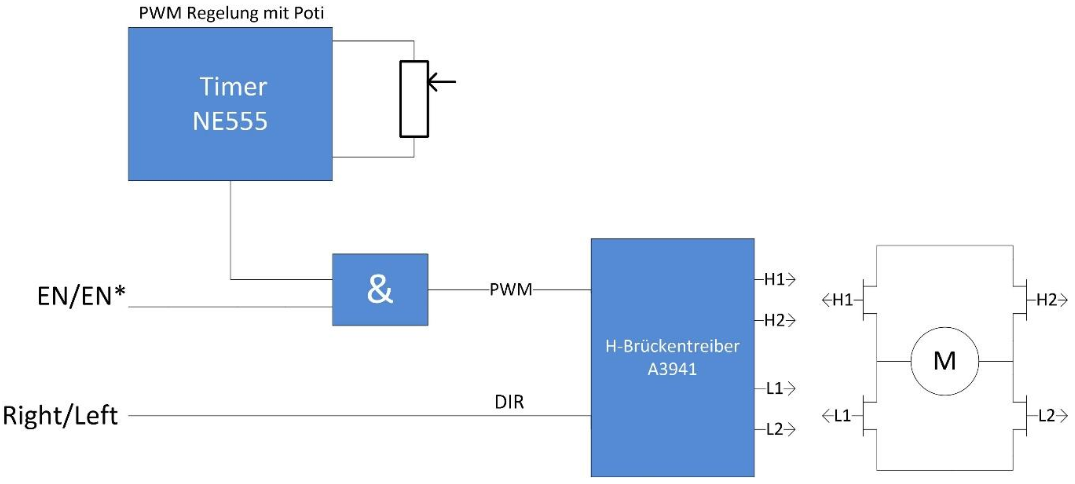
\includegraphics[width=0.75\textwidth]{src/dc/fig/timer_block.png}
	\caption{Blockschaltbild der Timerschaltung}
\end{figure}

\begin{figure}[h!]
	\centering
	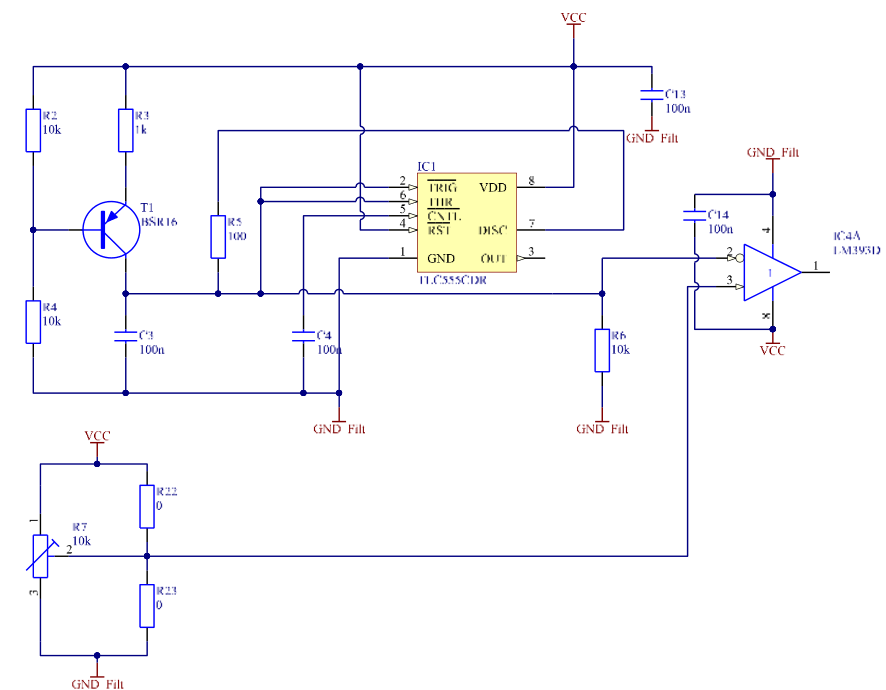
\includegraphics[width=0.75\textwidth]{src/dc/fig/timer_schematic.png}
	\caption{Timerschaltung}
\end{figure}

\subsection{PWM-Logik}
Mit dieser Logik kann eingestellt werden, ob das interne oder ein externes
PWM Signal verwendet werden kann. Wird auf das Switch-Signal eine Logische
0 gelegt, wird das interne PWM verwendet, bei einer Logischen 1 das externe
PWM. Das Switch Signal kann auch als ON/OFF Signal für das interne PWM
verwendet werden. Dazu muss nur das externe PWM Signal dauerhaft auf Ground
geschaltet werden. Auf diese Art kann zwischen internem PWM und keinem PWM
umgeschaltet werden. Diese Betriebsart wird im Moment verwendet.

Die Zehnerdiode am Ausgang wird benötigt, um das Ausgangssignal auf den
Logikpegel des A3941 zu senken. Die 400x IC Reihe kann mit bis zu 18V
betrieben werden und gibt auch annähernd diese Spannung wieder aus. Da der
A3941 maximal einen Logikpegel von 6.5V verträgt, muss die Spannung
gesenkt werden.

\begin{figure}[h!]
	\centering
	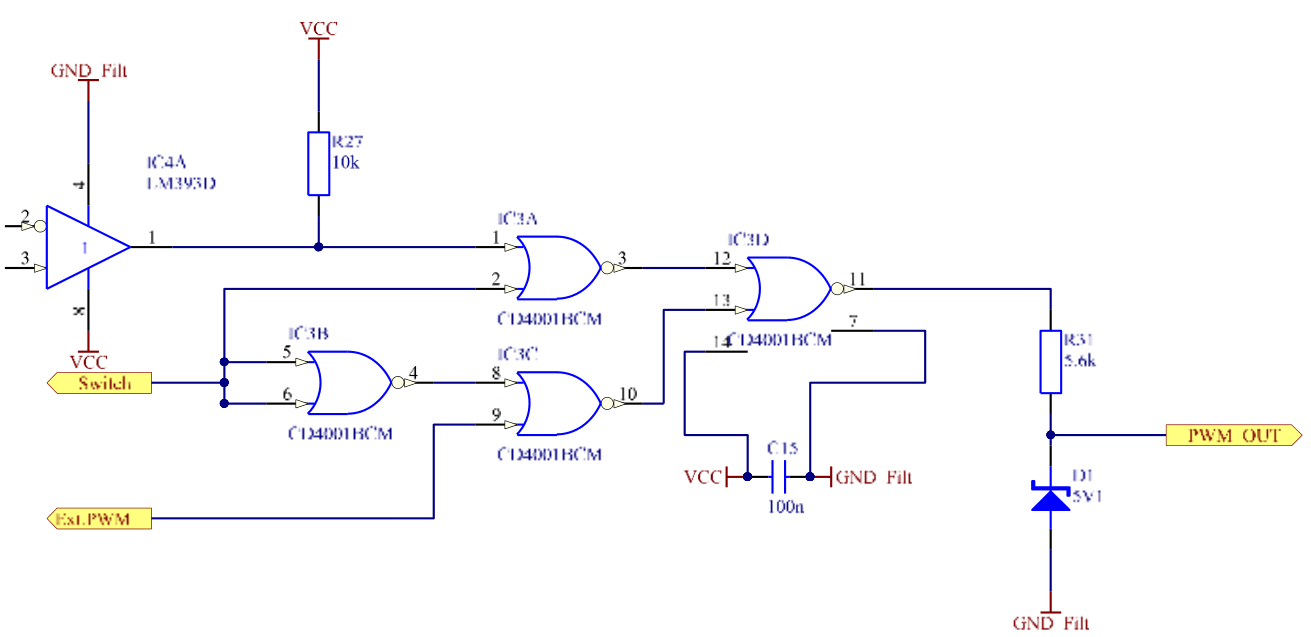
\includegraphics[width=0.75\textwidth]{src/dc/fig/pwm_schematic.png}
	\caption{Timerschaltung}
\end{figure}


\subsection{Ansteuerung}

